% Drawing a graph
% Author: Stefan Kottwitz
% https://www.packtpub.com/hardware-and-creative/latex-cookbook
\documentclass[border=10pt]{standalone}
\usepackage{tkz-graph}
\GraphInit[vstyle = Shade]
\tikzset{
  LabelStyle/.style = { rectangle, rounded corners, draw,
                        minimum width = 2em, fill = yellow!50,
                        text = red, font = \bfseries },
  VertexStyle/.append style = { inner sep=5pt,
                                font = \Large\bfseries},
  EdgeStyle/.append style = {->, bend left} }
\thispagestyle{empty}
\begin{document}
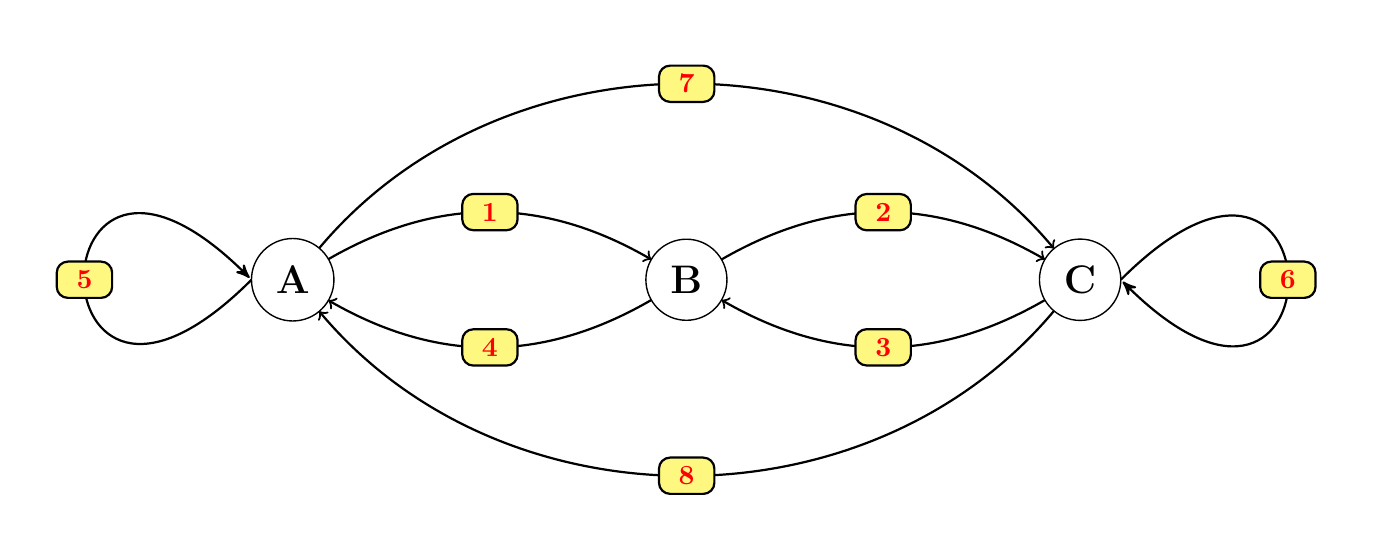
\begin{tikzpicture}
  \SetGraphUnit{5}
  \Vertex{B}
  \WE(B){A}
  \EA(B){C}
  \Edge[label = 1](A)(B)
  \Edge[label = 2](B)(C)
  \Edge[label = 3](C)(B)
  \Edge[label = 4](B)(A)
  \Loop[dist = 4cm, dir = NO, label = 5](A.west)
  \Loop[dist = 4cm, dir = SO, label = 6](C.east)
  \tikzset{EdgeStyle/.append style = {bend left = 50}}
  \Edge[label = 7](A)(C)
  \Edge[label = 8](C)(A)
\end{tikzpicture}
\end{document}
